%% Template Elsevier for Neuroimage

%% Use the option review to obtain double line spacing
\documentclass[authoryear,preprint,review]{elsarticle}
%\usepackage[framed,numbered,autolinebreaks,useliterate]{mcode}
\usepackage[framed,autolinebreaks,useliterate]{mcode}
\usepackage{natbib}
\usepackage{amsmath}
%\usepackage{lineno}
\usepackage{rotating}
\usepackage{hyperref}
\usepackage{amssymb}
\usepackage{amsfonts}
\usepackage{graphicx}
%\usepackage{algorithm2e}
%\usepackage{algorithmic}
%\usepackage{todonotes}

\journal{Neuroimage}
%\usepackage{color} 

\begin{document}

% Title must be 150 words or less
\begin{frontmatter}
%\title{Multiscale analysis of statistical parametric connectomes in resting-state fMRI}
\title{To Scrub Or Not To Scrub: The Impact Of Scrubbing On Resting-­State Connectivity In Alzheimer Progression}
\author[a,b]{Christian~Dansereau}
\author[a]{Pierre~Orban}
\author[a,b]{Pierre~Bellec\corref{cor1}}
\ead{pierre.bellec@criugm.qc.ca}
\cortext[cor1]{Corresponding author}
\address[a]{Centre de Recherche de l'Institut Universitaire de G\'eriatrie de Montr\'eal, Montr\'eal, CA}
\address[b]{D\'epartement d'Informatique et de recherche op\'erationnelle, Universit\'e de Montr\'eal, Montr\'eal,
CA}


% Please keep the abstract between 250 and 300 words
\begin{abstract}
%Exploring the association between connectomes and phenotypes is a ``needle in a haystack'' problem: very many connections to test, and potentially very few connections with high effects. The need to correct the significance of individual tests for the number of connections being tested hinders the sensitivity of the detection. A common approach to limit this multiple comparison problem is to only consider connections between about 100 brain parcels, instead of every pairs of voxels, which greatly reduces the number of connections and tests. Larger parcels may still average out highly spatially specific effects, and be overall detrimental to the power of statistical detection even after factoring in the gains in dimensionality. This work proposes a framework to systematically assess the impact of the number of parcels (scale) on the connectome-wide detection of associations with phenotypes. The detection of associations is achieved with a common mass univariate general linear model, applied independently at 
each connection. This procedure is repeated on a multiscale atlas of resting-state networks comprising anywhere from 5 to 400 networks, derived through a bootstrap analysis of stable hierarchical clusters. The multiple comparison problem is addressed at each scale independently, using variants of the false-discovery rate. An omnibus permutation test is implemented to reject the global null hypothesis of no association across all scales. We present both theoretical and empirical results supporting the fact that, when the global null is rejected, the false-discovery rate is well controlled both within and across scales using the proposed procedure. On simulations, we show that the optimization of scale can be used to achieve excellent sensitivity when detecting group differences in large samples (50 individuals per group), and good sensitivity in moderate samples (20 individuals per group). We applied the method on three different datasets with varying sample size: a group difference between blind subjects and 
sighted controls, a group difference between patients with schizophrenia and normal controls, and finally a longitudinal difference of resting-state connectivity pre and post learning practice of a motor task. Significant discoveries were made on all three datasets, and the results had excellent face validity: the main loci of changes fitted well with a priori from the literature. In addition, the multiscale method performed better than current state-of-the-art techniques such as network-based statistics or the multivariate distance matrix regression, both on simulations and real datasets. Taken together, our evaluations demonstrated that the multiscale general linear model on connectomes is a powerful tool to mine the association between connectivity and phenotypes.

Brain motion has been shown to introduce undesirable artifact in functional magnetic resonance imaging (fMRI) signal. A recent study by Power and coll. \citep{power2012} has demonstrated that even a small motion can seriously distort the measures of resting­state fMRI connectivity. The same work introduced a procedure called scrubbing to reduce the impact of motion. The scrubbing consists of removing the time frames with excessive motion, and it has been evaluated with fMRI collected mostly on children and adolescents. The behavior of scrubbing has however not been thoroughly tested in a population of young healthy adults, who tend to move less than children. In this study, we aimed to (1)characterize the typical distribution of the amount of motion in a young healthy adult population; (2)quantify the motion­related bias in resting state as a function of the amount of motion and (3)evaluate how the scrubbing impacts the motion­related bias depending on the amount of motion.

\end{abstract}

%-- 
\begin{keyword}
fmri \sep general linear model \sep functional parcellation \sep multiple comparison \sep false discovery rate \sep multiscale analysis \sep connectome
\end{keyword}
\end{frontmatter}

% Unique number for each line
%\linenumbers
%\listoftodos

\section*{Highlights}

\begin{itemize}
\item etc
 %\item The impact of the number of nodes, or scale, on the sensitivity of a connectome-wide association study is systematically evaluated.
 %\item A procedure is presented that controls the false-discovery rate within- and between scales.
 %\item The technique is evaluated on a simulation of multiscale changes in connectome organization.
 %\item The technique is applied on three different datasets, for which there is a good a priori knowledge on the underlying connectivity changes.
 %\item Several recent procedures for connectome-wide association are compared.
\end{itemize}

\section{Introduction}

% Magic paragraph
%% Connectome-phenotype association: choice of units is critical. 
%% Here multiscale exploration to (1) gain power; (2) demonstrate how multiscale CWAS can help explore the data.
\paragraph{Main Objective} 
%Brain connectivity in functional magnetic resonance imaging (fMRI) has been found to be a sensitive marker in a wide variety of neurological disorders \citep{Greicius2008}. Rather than focusing on a limited set of \emph{a priori} regions of interest, a recent trend is to systematically test for association between every possible brain connection (called a connectome) and the disease, or more generally a phenotypic trait of interest \citep{ShehzadInPress}. Such connectome-wide association study (CWAS) however raise an enormous multiple comparison problem: with $10^3$ brain parcels, there are about $10^6$ connections between parcels to test. When a massive number of univariate tests are performed, it becomes difficult to simultaneously reach acceptable rates of false positives (specificity) and false negatives (sensitivity). The number of multiple comparisons can be reduced by using less, bigger parcels, but then effects that are highly specific of small anatomical locations may get lost. Besides these statistical concerns, examining and interpreting all findings in a connectome quickly becomes challenging when the number of parcels gets large. How to choose the number of brain parcels (or scale) for a CWAS thus appears as a critical choice with implications both on the statistical power and the interpretability of a CWAS. The main objective of this work was to propose a statistical framework to perform a CWAS at multiple scales, instead of relying on a single parcellation, such that the impact of the spatial resolution can be assessed and optimized. 
\begin{itemize}
 \item Motion create artefact in fmri.
 \item Replication of the Power findings
 \item Does the connectivity is impacted similarly in elderly and demented population
 \item Do we gain at having cleaner data or to have more data of poorer quality
\end{itemize}


\paragraph{Impact of motion on rs-fMRI} 
-Detail the impact of motion on connectivity maps and the location of various motion artefacts, the sources of motion can be caused by motion (head motion due to muscle twitchs) per say but also by indirect causes like heart beat ans respiration.

\paragraph{Introduction to FD and justification for using this measure} 

\paragraph{Introduction to scrubbing} 
Even a mild amount of subject's motion can introduce marked artifacts in functional magnetic resonance imaging (fMRI) resting-state connectivity. In order to reduce these artifacts, \cite{power2012} proposed to remove the time frames with excessive motion, a technique called scrubbing. We aimed to (1) characterize the impact of motion on resting-connectivity in cognitively normal elderly (CNE) participants as well as patients with mild cognitive impairment (MCI) and dementia of the Alzheimer's type (DAT), and, (2) evaluate how the scrubbing impacts our ability to detect differences in connectivity between groups (CNE, MCI, DAT).

\paragraph{Classical method for motion artefact correction}
Classical method used to deal with motion specifically (coregistration, regression of motion parameters, voltera (Friston) 

\paragraph{Global method for artefacts correction} 
What are the other method used to correct global artefacts (COMPCOR,CORSICA (Bellec),GLOBAL SIGNAL) (Chao-Gan Yan)

\paragraph{Resting-state connectivity as a biomarker for AD} 

\paragraph{scrubbing impacts our ability to detect changes in dementia progression} 
-Could scrubbing impacts our ability to detect changes in muticentric studies investigating progression of dementia?


%We hypothesized that some data-dependent scale would give an optimal statistical power by achieving a trade-off between the degree of functional specialization (which is maximal at high scales) versus the amount of multiple comparisons (which is minimal at low scales). We also hypothesized that the multiscale analysis would provide an efficient way to make sense of the results of a CWAS, as low scale would provide an overall picture of the associations, and guide the exploration of detailed associations at higher scales.
%When brain parcellations are generated with a data-driven cluster analysis \citep{Bellec2010c,Bellec2013}, the low scales (10s of parcels) involve large-scale networks and a very limited number of multiple comparisons. At the other end of the spectrum, high scales (100s or even 1000s of parcels) involve anatomically segregated regions that can capture effects specifically impacting highly specialized systems, but come at the price of a very large number of multiple comparisons. 

%\paragraph{Parcellations and testing} 
% brain parcellatione m
% Region growing -> Lu, Thirion
% The Network based statistics approach of Zalesky et al. 
%Clearly, the simplest way to reduce the multiple comparisons in a CWAS is to reduce the number of brain parcels. This can be achieved by averaging time series on a set of brain regions delineated based on anatomical landmarks such as the AAL template \citep{Tzourio-Mazoyer2002}, e.g. the study of \cite{Wang2007} on Alzheimer's disease. Rather than using anatomical parcels, it is possible to build data-driven brain parcels that optimally capture the underlying spatial correlation structure of the data at the voxel level \citep{Bellec2006,Shen2010,Craddock2011,Blumensath2013}. It was shown in the context of task activation detection that using data-driven brain parcellation instead of voxels could result into improved sensitivity in mass univariate GLM analysis \citep{Lu2003,Thirion2006} as well as multivariate prediction \citep{Xu2010}. However, even with a relatively small number of brain parcels $N=100$, there are still about $5000$ multiple comparisons. The work of \cite{Zalesky2010b} thus proposed to use uncorrected threshold on the individual $p$-values, but then to identify to which extent the connections that survive the test are interconnected. This extent measure is compared against what could be observed under a null hypothesis of no association, implemented through permutation testing. As the authors noted themselves, this strategy only offers a loose control of false-positive rate at the level of a single connection, but can be used to reject the possibility that a group of significant findings could be observed by chance in the FWE sense. 

%\paragraph{Multiscale parcellations} 
% Choice of the parcels
% Paper of Kiviniemi on multiscale ICA

% Nothing for mass univariate testing.
% Paper of Thirion etc on multiscale prediction http://www.sciencedirect.com/science/article/pii/S0031320311001439
%Few works have investigated how to select the parcels, and in particular their number, in order to maximize the statistical power of a GLM analysis. While adding brain parcels will mechanically improve the accuracy of the approximation of fMRI fluctuations, when comparing time series at the voxel level and average time series on parcels \citep{Craddock2011}, such an increase also comes at the cost of extra multiple comparisons. This issue is exensively discussed by \cite{Meskaldji2011}, who  proposed an adaptative method resulting into substantial gains in sensitivity when using low-dimensional parcels. Independently, the work of \cite{AbouElseoud2011} systematically explored the impact of scale (number of components) on the ability of a dual-regression ICA analysis, when trying to discriminate between a group of patients suffering from unmedicated seasonal affective disorder from normal healthy controls. The authors concluded that scale 70 (with about 45 resting-state networks, the other ones being noise or unidentified components) increased the number of discoveries by a factor of three. The authors also noted that higher scales may result in higher rates of false-positives, as more components also meant more multiple comparisons. The authors did not investigate the implications that testing many scales, which is another form of multiple comparisons, would have in terms of the control of false positives.

% Anat vs functional parcels \citep{Shirer2012}
\paragraph{Specific objectives} 
% Obective 1: Develop a statistical framework for scale optimization in statistical parametric connectomes. 
% Objective 2: test empirically the specificity/sensitivity of the approach (??and compare it to ??)
% Objective 3: Demonstrate empirically the benefits of scale optimization. 
% % Multiscale parcellationt
% visualization. Help to guide the interpretation. Yeo, Kelly, Orban et al. 2014.
%In this paper, our main objective was to develop a novel statistical framework, called multiscale GLM-connectome, to systematically perform a CWAS at multiple spatial scales, while providing an explicit control of the FDR within and across scales. \emph{Insert very quick overview of the GLM-connectome method}. Our second objective was to validate and evaluate the multiscale GLM-connectome method. In particular, we compared the behaviour of the multiscale GLM-connectome when implemented with two variants of algorithms controlling the false-discovery rate \citep{Benjamini1995,Hu2010}, as well as the NBS \citep{Zalesky2010b} and the MDMR \citep{ShehzadInPress}.

\begin{itemize}
 \item Motion artefact and it's impact on functional connectivity
 \item Motion distribution in ECN, pMCI and pDAT
 \item Impact of scrubbing on the connectivity of each populations
 \item Impact of scrubbing on our discriminative power between populations
\end{itemize}



\paragraph{Real datasets}
We evaluated the multiscale GLM-connectome on three real datasets: (1) a study on patients suffering of blindness, compared to sighted controls (referred to here as the BLIND dataset, with a small sample size, $n=?$); a study of motor learning, where resting-state data was acquired before and after learning of a new motor task (referred to here as the MOTOR dataset, with a moderate sample size, $n=?$), and; (3) a study comparing patients suffering from schizophrenia with healthy control subjects (referred to here as the SCHIZO dataset, with a large sample size, $n=?$). These three datasets where chosen to assess if GLM-connectome would be able to uncover statistically significant effects in a variety of sample sizes. Also, there are strong a priori hypothesis for those three analysis: changes in the visual network for the BLIND dataset, in the motor network for the MOTOR dataset and a general dysconnectivity in the SCHIZO dataset. These a priori were useful to qualitatively assess the face validity of the technique. 



\section{Methods} 

\subsection{Data samples} 
\paragraph{Participants} %The SCHIZO dataset comprised 72 patients diagnosed with schizophrenia (58 males, age range = 18-65 yrs) and 74 healthy controls (51 males, age range = 18-65 yrs). The BLIND dataset was composed of 14 congenitally blind volunteers (10 males, age range = 26-61 yrs) and 17 sighted controls (8 males, age range = 23-60 yrs). The MOTOR dataset included 54 healthy young participants (33 males, age range = 19-33 yrs).

The paper studies 313 elderly adults with and without cognitive impairment of the Alzheimer type collected across 5 studies: ADNI2 study and 4 other studies based in Montreal, Canada (from the ADMTL consortium), for a grand total of 126 CNE participants, 133 patients with MCI, and 54 patients with DAT (see table \ref{dataset}).


\paragraph{Acquisition} %Resting-state scans were acquired on a 3T Siemens TrioTim for all datasets. \emph{Ethics approval ?? Where are the data coming from ?}. One single run was obtained per subject for either the SCHIZO or BLIND dataset while two runs were acquired in each subject for the MOTOR dataset, one immediately preceding and one following the practice on a motor task (see Supplementary Material) . For the SCHIZO dataset, 150 EPI blood-oxygenation level dependent (BOLD) volumes were obtained in 5 mns (TR = 2~s, TE = 29~ms, FA = 75\textdegree, 32 slices, voxel size = 3x3x4~mm$^3$, matrix size = 64x64, FOV = mm$^2$), and a structural image was acquired using a multi-echo MPRAGE sequence (TR = 2.53~s, TE = 1.64/3.5/5.36/7.22/9.08~ms, FA = 7°, 176 slices, voxel size = 1x1x1$mm^3$, matrix size = 256x256, FOV = 256x256$mm^2$). For the BLIND dataset, 136 EPI BOLD volumes were acquired in 5 mins (TR = 2.2s, TE = 30~ms, FA = 90\textdegree, 35 slices, voxel size = 3x3x3.2$mm^3$, gap = 25\%, matrix size = 64x64, FOV = 192x192$mm^2$), and a structural image was acquired using a MPRAGE sequence (TR = 2.3~s, TE = 2.91~ms, FA = ?\textdegree, 160 slices, voxel size = 1x1x1.2$mm^3$, matrix size = 240x256, FOV = 256x256mm$^2$). For the MOTOR dataset, 150 EPI volumes were recorded in 6 mins 40 s (TR = 2.65s, TE = 30ms, FA = 90\textdegree, 43 slices, voxel size = 3.4x3.4x3$mm^3$, gap = 10\%, matrix size = 64x64, FOV = 220x220$mm^2$), and a structural image was acquired using a MPRAGE sequence (TR = 2.3~s, TE = 2.98~ms, FA = 9\textdegree, 176 slices, voxel size = 1x1x1$mm^3$, matrix size = 256x256, FOV = 256x256$mm^2$).


We need to talk about what we sould say for the parameters not a lot of information is available ...


\subsection{Preprocessing} The datasets were analysed using the NeuroImaging Analysis Kit (NIAK\footnote{\url{http://www.nitrc.org/projects/niak/}}) version 0.12.14, under CentOS version 6.3 with Octave\footnote{\url{http://gnu.octave.org}} version 3.8.1 and the Minc toolkit\footnote{\url{http://www.bic.mni.mcgill.ca/ServicesSoftware/ServicesSoftwareMincToolKit}} version 0.3.18. Analyses were executed in parallel on the "Mammouth" supercomputer\footnote{\url{http://www.calculquebec.ca/index.php/en/resources/compute-servers/mammouth-parallele-ii}}, using the pipeline system for Octave and Matlab \citep{Bellec2012}, version 1.0.2. Brain map visualizations were created using MRICron software \cite{Rorden2007}. Each fMRI dataset was corrected of inter-slice difference in acquisition time and the parameters of a rigid-body motion was estimated for each time frame. Rigid-body motion was estimated within as well as between runs, using the median volume of the first run as a target. The median volume of one selected fMRI run for each subject was coregistered with a T1 individual scan using 
Minctracc (Collins et al. 1997), which was itself non-linearly transformed to the Montreal Neurological Institute (MNI) template (Fonov et al 2011) using the CIVET pipeline (Zijdenbos et al. 2002). The MNI symmetric template was generated from the ICBM152 sample of 152 young adults, after 40 iterations of non-linear coregistration. The rigid-body transform, fMRI-to-T1 transform and T1-to-stereotaxic transform were all combined, and the functional volumes were resampled in the MNI space at a 3 mm isotropic resolution. The “scrubbing” method of \cite{Power2012}, was used to remove the volumes with excessive motion with three cut-offs points: no scrubbing ($FD\geq0$), $FD\geq0.5$ and $FD\geq0.2$. A minimum number of 50 unscrubbed volumes per run, corresponding to $\sim 125$ s of acquisition for a TR of 2.5 seconds, was then required for further analysis. For this reason, some subjects were rejected from the subsequent analyses: 11 CNE, 13 pMCI and 3 pDAT for a scrubbing at $FD\geq0.5$ and 83 CNE 95 pMCI and 39 
pDAT for a scrubbing at $FD\geq0.2$ (see table \ref{table_scrubbimpact}). The following nuisance parameters were regressed out from the time series at each voxel: slow time drifts (basis of discrete cosines with a 0.01 Hz high-pass cut-off), average signals in conservative masks of the white matter and the lateral ventricles as well as the first principal components (95\% energy) of the six rigid-body motion parameters and their squares (Lund et al. 2006, Giove et al. 2009). The fMRI volumes were finally spatially smoothed with a 6 mm isotropic Gaussian blurring kernel. 

%\subsection{Functional connectivity maps}
% Introduce the concept of connectome and connectivity maps
%\label{sec_connectome}
%begin{center}
%------ Figure~\ref{fig_glm} about here ------\\
%\end{center}

%For each scale, and each pair of distinct networks $i$ and $j$, the between-network connectivity $y_{i,j}$ is measured by the Fisher transform of the Pearson's correlation between the average time series of the network. The within-network connectivity $y_{i,i}$ is the Fisher transform of the average correlation between time series of every pair of distinct voxels inside network $i$. The connectome $\mathbf{Y}=(y_{i,j})_{i,j=1}^R$ is thus a $R\times R$ matrix. Each column $j$ (or row, as the matrix is symmetric) codes for the connectivity between network $j$ and all other brain networks, or in other word is a full brain functional connectivity map. See Figure \ref{fig_SPC}\textbf{a-b} for a representation of a parcellation and associated connectome. Connectomes are generated independent at each scale. See Appendix \ref{app_connectome} for a more formal description of the connectome generation.


%\subsection{Statistical parametric connectome}
%\label{sec_spc}
%For a scale with $R$ parcels, there are exactly $L=R(R+1)/2$ distinct elements in an individual connectome $\mathbf{Y}$. This connectome can be stored as a $1\times L$ vector, where the brain connections have been ordered arbitrarily along one dimension. When functional data is available on $N$ subjects, the group of connectomes is then assembled into a $N\times L$ array $\mathbf{Y}=(y_{n,l})$, where $n=1,\dots,N$ each code for one subject and $l=1,\dots,L$ each code for one connection. A general linear model (GLM) framework can then be used to test the association between brain connectivity and a trait of interest, such as the age or sex of participants. All of these $C$ explanatory variables are entered in a $N\times C$ matrix $\mathbf{X}$. The variables are typically corrected to have a zero mean across subjects, and an intercept (i.e. a column filled with 1) is added to $\mathbf{X}$. The GLM relies on the following stochastic model:
% \begin{equation}
% \label{eq_glm}
%  \mathbf{Y} = \mathbf{X}\mathbf{B} + \mathbf{E},
% \end{equation}
%where $\mathbf{B}$ is an unknown $C\times L$ matrix of linear regression coefficients and $\mathbf{E}$ is a $N\times L$ random (noise) multivariate Gaussian variable. As data generated from different subjects are statistically independent, and under an homoscedasticity assumption, the regression coefficients $\mathbf{B}$ can be estimated with ordinary least squares. For a given ``contrast'' vector $C$ of size $1\times C$, the significance of $C.B$ can be tested with a connectome of $t$-test $(t_{l})_{l=1}^L$, with associated $p$-values $(p_l)_{l=1}^L$. The quantity $p_l$ controls for the risk of false positive findings at each connection $l$. The GLM applied on connectomes is illustrated in Figure \ref{fig_glm}\textbf{c}. See Appendix \ref{app_glm} for the equations related to the estimation and testing of regression coefficients in the GLM.

%\subsection{False discovery rate}
% Present the different approaches for FDR
%\paragraph{The Benjamini-Hochberg FDR} In traditional (univariate) applications, a $p$ value below $0.05$ is considered as a solid evidence of an effect. For a given scale, there are however a large number $L$ of such tests on $p_l$ to perform. So even with a 5\% chance of a false positive at connexion $l$, in the absence of any effect one would report 5\% of the whole connectome as associated with a significant effect. The significance value applied on $p_l$ thus needs to be adjusted for this multiple comparison problem. We implemented two strategies for controling the false-discovery rate (FDR). The idea behind the FDR is not to strictly control the probability to observe at least one false positive (a quantity know as family-wise error, FWE), but rather to control the proportion of false positive amongst the findings. Note that controling for the FDR is not necessarily a more liberal attitude than controling for the FWE: if the global null hypothesis is verified, i.e. all discoveries are false positive, then the FDR is exactly the FWE. In the presence of true discoveries, however, the FDR procedure tolerates in general more noise than a FWE approach. The actual number of false discoveries will dependend on the amount of signal (true positive) present in the data, and is therefore a context-dependent question. The popular Benjamini-Hochberg (BH) procedure was proposed to control the FDR $q$ to an acceptable level $\alpha$ \citep{Benjamini1995}. This algorithm was designed for independent tests, but it has been shown to have a satisfactory behaviour even in the presence of positive correlation between the tests $p_l$ \citep{Benjamini2001}. 

%\paragraph{The group FDR} A documented limitation of the BH procedure is its lack of sensitivity to sparse signals \citep{Hu2010}. If only a small subset of brain parcels show some significant effects, the maps of low signal will contribute a lot of noise and the FDR threshold that is set globally will be quite conservative. A connectome has a natural structure:  each column of the SPC represent a full brain connectivity map, where the parcel associated with the column acts like the seed (see Figure \ref{fig_SPC}\textbf{a}). Some regions of the brain are likely to be particularly impacted by the trait of interest, and be associated with many discoveries, while others will be associated with very few or even no discoveries. This means that some columns in the connectome will be associated with much more discoveries than others. These columns thus represent natural groups of tests within the full connectome, yet this structure is completely ignored in the BH procedure. Several solutions have recently been proposed for this issue \citep{Efron2008,Cai2009,Hu2010,Benjamini2011}. We focused in this work on the least-slope variant of the group FDR procedure proposed by \cite{Hu2010}. The idea of the group FDR is to first assess the presence of signal in each column (map) independently, and then re-weight the original $p$-values based on the presence (or absence) of promising signal. It was shown that both the group FDR procedure controls asymptotically the global FDR for independent tests, yet they are expected to be much more sensitive than BH for sparse signals \citep{Hu2010}. These procedure were also reported to behave correctly in the presence of positive dependency between tests, although no analytical properties were derived in that case. We investigated experimentally the differences between the BH and group FDR procedures, both on simulated data (Section \ref{sec_simus}) and real data (Section \ref{sec_comparison}). The Appendix \ref{app_fdr} provides a formal description of both the global and the group FDR algorithms. Note that all these procedures have been made publicly available as a Matlab/Octave code\footnote{\url{http://code.google.com/p/niak/source/browse/trunk/commands/statistics/niak_fdr.m}}.
% 

%\subsection{Functional parcellations} The first step to build such a connectome is to select a parcellation of the brain, with $R$ networks. In this work, we used functional brain parcellations, aimed at defining groups of brain regions with homogeneous time series. A number of algorithms have been proposed with additional spatial constraints, to ensure that the resulting parcels are spatially connected \citep{Lu2003,Thirion2006,Bellec2006,Craddock2011}. However, from a pure functional viewpoint, the spatial constraint seems somewhat arbitrary, as functional units in the brain at low resolution encompass distributed networks of brain regions with homotopic regions often being part of a single parcel \citep{DeLuca2006,Damoiseaux2006}. Some works have thus used distributed parcels as the spatial units to measure functional brain connectivity, e.g. \citep{Jafri2007,Marrelec2008}. To generate the functional parcelations, we relied on a recent method called ``Bootstrap Analysis of Stable Clusters'' (BASC), which can identify consistent functional parcels for a group of subjects \citep{Bellec2010c}, using a hierarchical cluster with Ward's criterion both at the individual and the group levels. Details regarding the method can be found in \cite{Bellec2010c}. The functional parcels can be generated at any arbitrary resolution (within the range of the fMRI resolution), and we considered only clusters generated at the group level.

\paragraph{Parcellation}
Functional brain parcellation into 100 regions was obtained from an independent reference dataset of healthy adults from the 1000 functional connectome project (Cambridge cohort, parcelation available here \ref{}). To do so the spatial dimension of the independent individual fMRI dataset was reduced to 957 regions using a region-growing algorithm \cite{Bellec2006} and final network decomposition was obtained using BASC \cite{Bellec2010c} a bootstrap method to identify stable networks at various scales.

\subsection{Connectome and functional maps}
For each run, the correlation matrix was generated base on the time series averaged on the parcellation of an independent dataset mention previously (Cambridge 100 parcels). For each subject, the connectomes were averaged across all runs. The following regions were selected based on the literature: posterior cingulate cortex (PCC) a central node of the default mode network and the left middle temporal (MT) part of the dorsal attention network. Finally, the average voxelwise functional connectivity maps were generated for each selected region, i.e. Pearson's correlation corrected by the Fisher transform and averaged across all runs for each subject. The significance of the difference in connectivity between scrubbing level for each group was established using a t-test and a group false-discovery rate (FDR) procedure \cite{Hu2010} at $q<0.05$. To test the impact of scrubbing on our ability to detect differences in a contrast between groups, we tested the significance of the difference in mean connectomes at different levels of scrubbing within each group using paired t-tested and a group FDR procedure at $q<0.05$.

\subsection{Statistical analysis} %Brain parcellations were derived using BASC separately for each dataset, while pooling the groups (SCHIZO, BLIND) or runs (MOTOR), over a grid of scales: from 5 to 100 (step of 5), from 110 to 200 (step of 10), and from 220 to 400 (step of 20). By contrast, the NBS and MDMR procedures were implemented at two scales only: 10 and 100 parcels. The multiscale GLM-connectome (both BH and group FDR), as well as the NBS and MDMR procedures were implemented with the same parameters as those used on simulations (see Section \ref{sec_methods_simu}. For every contrasts, the group model included the age of participants and the average frame displacement of the runs involved in the analysis (two covariates of frame displacement were used in the MOTOR dataset), corrected to a zero mean. The contrast of interest was on a dummy covariate coding for the difference in average connectivity between the two groups for SCHIZO and BLIND, and on the intercept (average of the difference in connectivity pre- and post-training) for the MOTOR dataset.

\paragraph{Power analysis} 
Group differences (ECN, pMCI and pDAT) for 3 preprocessing stategy (no scrubbing, scrubbing FD > 0.5 and scrubbing FD >0.2) were investigated using t-tests in a linear model for ten point-to-point connections selected based on a literature review including covariates to model site-specific bias (false-positive rate $p<0.05$). Namely the point-to-point connections are: (1)PCC/PCUN, (2)dMPFC/dMPFC2, (3)IPL/SFGr, (4)aMPFC/PCUN, (5)SFGr/FUS, (6)PCC/PCUNm, (7)IPL/dMPFC3, (8)PCC/MTL, (9)IPL/MTL, (10)aMPFC/MTL. The detection power is computed using a t-test of each connection (p<0.05) replicated 10,000 times using random subsamples of 70\% of each group. Explanatory variables included age and gender. Consistent differences for data generated on Philips and Siemens scanners were identified using model averaging (Willer et al., 2010).


\section{Results} 

\subsection{Motion distribution in ECN, pMCI and pDAT} 
A good overlap in the FD distribution across groups has been observed, the effect of scrubbing reduce the spread of the distribution and center the average FD around 0.2 for scrubbing with a threshold $FD\geq0.5$ and 0.1 for a threshold of $FD\geq0.2$.There is therefore no apparent differences in FD for the three populations. 90\% of subjects survived the exclusion criteria of a minimum of 50 frames after scrubbing at $FD\geq0.5$ and 30\% surviving rate with an aggressive scrubbing of $FD\geq0.2$.

\subsection{Impact of scrubbing on the connectivity}
\paragraph{Global impact of scrubbing}
\paragraph{Population specific impact of scrubbing}

\subsection{Impact of scrubbing on our discriminative power between populations}
\paragraph{Pair to pair connections}
\paragraph{Detection power for every scrubbing strategy}

% a changer par christian
% -How scrubbing impact detection of differences bases on p2p connections
% The AFD varied widely in the sample, from 0.05 to 0.35+ see Fig.1A for the complete distribution and the three groups. Fig.1B shows that scrubbing reduced the differences in residual FD between groups, yet the differences remained significant even at very conservative cut-off of 0.2. Note that no subjects in the "high motion" group could be included at (FD≤0.2) due to an insufficient number of volumes surviving scrubbing. In order to ease the reading we will present the connectivity map of the two classic functional networks namely the default mode network generated with a seed in the posterior cingulate cortex (PCC) (Fig.2 & 3) and the dorsal attention network obtained with a seed in the left middle temporal (MT) region (Fig.4 & 5). For more detailed results of all connections see connectivity matrices in supplementary material. A significant bias in resting­state connectivity was observed in all group comparisons, with a trend towards small positive correlations and a larger standard deviation across subjects for an increasing level of motion (Figs. 2 & 4). Fig.3 & 5 shows that the scrubbing had only a very mild impact on the average connectome for all groups: effects reached significance in the areas affected by motion for FD≤0.5 and FD≤0.2 in the "moderate motion" group regrettably not enough to bring back a functional map similar to the target low motion group. Furthermore, only 17 subjects out of 148 in this group had enough volumes surviving scrubbing at FD≤0.2 to enter this analysis.
% A wide range of motion level was observed in the sample. An arbitrary cut-off was used to separate the population into "moderate" and "high" motion groups". A bias in connectivity measures was observed between the “moderate” and “high” motion groups (Fig. 1A). The 0.5 scrubbing significantly improve connectivity strength for both groups in the network and reduce connectivity with anti-correlated regions (Fig. 1B). Despite a moderate loss of subjects using the 0.5 scrubbing due to insufficient remaining data < 50 frames, the gain in data quality translated into an increased detection rate for group differences in all tested connections.


%\paragraph{Spatial distribution of significant discoveries} Discovery percentage maps revealed which parcels were associated with the largest amount of discoveries, and more specifically the proportion of significant connections for any given parcel, in all three real datasets (See Figure \ref{fig_perc_disc_maps}). Results for scales 10 and 100 were reported for all four explored techniques (GLM-connectome with BH and group FDR, MDMR and NBS), when applicable. Significant effects were found for all contrasts both at scales 10 and 100 with the group FDR variant GLM-connectome. Widespread effects were observed for the SCHIZO dataset at both cortical and subcortical levels. Parcels with the highest number of connections being altered were found the temporal lobe, the prefrontal cortex, the medial temporal lobe and the basal ganglia. The between-subjects contrast in the BLIND dataset revealed more localized effects in the occipital cortex, and to a lesser extent in the temporal and premotor cortices. Finally, the within-subject contrast in the MOTOR dataset identified significant effects within an extended cortico-subcortical motor network (sensorimotor and premotor areas, basal ganglia and spinocerebellum). Note that the effects in the basal ganglia and cerebellum can be seen in Supplementary Figure \ref{fig_motor_subcortical}, as Figure \ref{fig_perc_disc_maps} only shows cortical surface representations.

%\paragraph{Comparison between detection techniques} Discovery percentage maps further made clear that the BH FDR procedure showed less significant effects than the group FDR. Yet, apart from the contrast in the BLIND dataset at scale 10 that did not reveal any significant effect, the results were highly consistent between the two procedures for all other contrasts. The MDMR analysis gave significant results for scales 10 and 100 in the SCHIZO dataset as well as scale 100 but not 10 in the BLIND dataset. Again, the spatial loci of significant change in functional connectivity were consistent with the GLM-connectome analysis. Of note, MDMR cannot be used to assess within-subject contrast and therefore was not applied to the MOTOR dataset. The NBS technique only revealed significant effects for the SCHIZO dataset. In this specific case, the group FDR analysis was associated with less discoveries than the NBS analysis, yet the overall spatial distribution of maximal effects was similar between techniques. Besides, it is interesting to note that some contrasts that did not show any significant effects using NBS with a $p < 0.01$ showed spatially consistent effects when tolerating a very liberal $p < 0.2$ (see Supplementary Figure \ref{fig_mdmr_p_0.2}). Overall, these results indicated a good consistency across techniques in localizing parcels with maximal effects, but also clearly highlighted the higher detection rate of the GLM-connectome with group FDR approach over the other ones.

%\paragraph{Seed-based maps of $t$-statistics} Discovery percentage maps identified which parcels were associated with many significant discoveries. Yet, these maps did not characterize which specific connections were identified as significant, nor the direction of the effect is (i.e. an increase vs a decrease in connectivity). We decided to illustrate how the results can be explored at this finer level of granularity for the SCHIZO dataset only, because we obesrved widespread changes in functional connectivity. The percentage of discovery maps were used to select a number of seed parcels showing maximal effects, i.e. networks found in the temporal and prefrontal cortices, the medial temporal lobe as well as the basal ganglia (see Figure \ref{fig_eff_maps}, see also Supplementary Figure \ref{fig_xxx}). For each parcel, a FDR-corrected t-test map associated with the contrast of interest was generated. These $t$-maps revealed that the alterations in functional coupling in schizophrenia essentially took the form of a decrease in connectivity, in particular for connections linking temporal, prefrontal and occipital regions. By contrast, the basal ganglia showed an increase in functional connectivity with occipital and temporal areas in schizophrenia. Functional connectivity was also increased between the hippocampus/amygdala and the medial prefrontal cortex. Of note, discoveries made with large networks, at scale 10 (e.g., basal ganglia), led to similar conclusions as the discoveries made with local regions at scale 100 (e.g., thalamus).   

\section{Discussion}

\subsection{Findings FD distribution}
%The effects found on the real datasets were consistent with the existing literature. First, schizophrenia has been defined as a dysconnectivity syndrome, with aberrant functional interactions between brain regions being a core feature of this mental illness \citep[for reviews, see]{Calhoun2009,Pettersson-Yeo2011,Fornito2012}. As found here, alterations in connectivity were widespread and mostly decrease in connectivity in patients, with the strongest effects in the temporal and prefrontal cortices. Increases in connectivity were also observed, for instance in the basal ganglia, in line with (REF). Second, resting-state fMRI studies have previously shown that congenital blindness is associated with a reorganization of the interactions between the occiptial cortex and the rest of the brain, and in particular the auditory and premotor cortices (Liu et al. 2007; Qin et al., 2013, 2014), consistent with our findings. Finally, our results are consistent with the observation that brain activity at rest is modulated by previous intensive motor practice \citep{Albert2009,Vahdat2011, Sami2013}. Together, our findings on real datasets had good face validity, and suggested that the GLM-connectome could likely be successfully applied to a variety of clinical or experimental conditions.

\paragraph{Differences in connectivity between young adult and elderly subjects}
Mention the increase connectivity in elderly subjects (reduce amount of negative correlations)


\subsection{Discriminative power impacted by scrubbing}
Mention the quality of the data and if it's impact on our ability to discriminate groups (CNE, pMCI, pDAT)

%\subsection{Comparison with other methods}
%With the simulation scenarios we tested, the multiscale GLM-connectome method (with group FDR) emerged as the best option in terms of sensitivity. The three real datasets featured different sample sizes: around 15 and 70 participants per group for between-subject comparisons (BLIND and SCHIZO, respectively) and around 50 participants for the within-subject comparison (MOTOR). In addition, while one contrast was expected to involve very distributed systems (SCHIZO), others were anticipated to show fairly localized effects (BLIND and MOTOR). Despite the diversity of those configurations, the comparison between methods on those real datasets led to rather similar conclusions. Overall, the multiscale GLM-connectome (with group FDR) appeared to be the most sensitive technique, as compared to the BH FDR, NBS or MDMR. In most cases, this observation was true both at low (10) and high (100) scales. While FDR approaches revealed significant effects in all three datasets, MDMR and NBS techniques only provided significant findings in a few cases. One major caveat when comparing GLM-connectome with other techniques such as NBS or MDMR is that they were not designed to answer the exact same questions, nor do they control for statistical risk in similar ways. In particular, MDMR and NBS work well at higher resolutions, up to voxel-level inferences for MDMR. By contrast, the GLM-connectome behaved particularly well at relatively low scales (tens of parcels), but we expect it to perform poorly at voxel resolution. An interesting future extension of this work would be to integrate MDMR to perform the within-scale testing in our multiscale framework instead of the FDR procedure. We would however need to establish first how statistical risk propagates across scales using MDMR.  

%\subsection{Beyond scale selection: choice of the brain parcellation}
%Although the impact of the number of parcels on CWAS sensitivity has been extensively investigated in this work, we only briefly examined how the choice of parcels, and not just their number, could impact statistical sensitivity. We could for example have used random parcellations, like \citep{Zalesky2010}, or a parcellation based on anatomical landmarks such as the AAL atlas \citep{Tzourio-Mazoyer2002}. From our results on simulations, it seems clear that dramatic differences in statistical power can be achieved at a given spatial scale, if a set of parcels is best adapted to the spatial distribution of an effect. Following an idea initially explored in \citep{Thirion2006}, it may even be possible to relax the constraint of identical parcels across subjects, by matching different individual-specific parcels and use this correspondence to run group-level CWAS analysis. We believe that important improvement in sensitivity could be gained from the optimization of the parcellation scheme, rather than scale, and this represents an important avenue for future research.

 

\subsection{Other connectivity metrics}
Introduce the stability maps as a potential metric providing more stable results and more robusts to motion and other artefacts

%The only connectivity metric considered here was the Pearson's correlation coefficient between fMRI time series of a pair of brain parcels. There are however many other metrics that have been proposed in the literature, see e.g. \citep{Smith2010}. The GLM-connectome pipeline can be applied to any connectivity metric, provided that (1) it can be estimated on networks of various sizes, and; (2) the distribution of the metric at the group level does not depart markedly from the assumptions of the basic GLM we used: Gaussian, independent and identically distributed (homoscedastic) residuals. In its current implementation, the GLM-connectome pipeline supports partial correlation \citep{Marrelec} (after Fisher transform), correlation based on a subset of volumes of an individual run, difference in correlation between two subsets of volumes of an individual run, as well as psychophysiological interaction in an individual run. It is also possible to combine multiple runs per subject, e.g. to derive the difference in connectivity between two time points. 

\section{Conclusions}
Motion introduces a systematic bias in the measures of resting-­state connectivity even in young healthy adults. The scrubbing procedure does not allow reducing substantially this bias unless it is performed aggressively, in which case the vast majority of subjects are lost. These results unfortunately question the usefulness of the scrubbing procedure for short resting­-state fMRI acquisition (5 min). More work is needed to study the impact of scrubbing for longer acquisitions (10­20 mns).

\section{Acknowledgments}
Parts of this work were presented at the 2013 annual meetings of the organization for human brain mapping \citep{?}, as well as the  Alzheimer's Association International Conference (AAIC) (2014) (Copenhagen) \citep{?}. The authors are grateful to the members of the 1000 functional connectome consortium  and the ADNI2 initiative for publicly releasing there dataset. The computational resources used to perform the data analysis were provided by ComputeCanada\footnote{\url{https://computecanada.org/}} and CLUMEQ\footnote{\url{http://www.clumeq.mcgill.ca/}}, which is funded in part by NSERC (MRS), FQRNT, and McGill University. This project was funded by NSERC grant number RN000028, a salary award from ``Fonds de recherche du Qu\'ebec -- Sant\'e'' to PB as well as a salary award by the Canadian Institute of Health Research to CD.

\section*{References}

\bibliographystyle{elsarticle-harv}
\bibliography{pbellec}

\section*{Figure Legends}

\begin{figure}[!ht]
\begin{center}
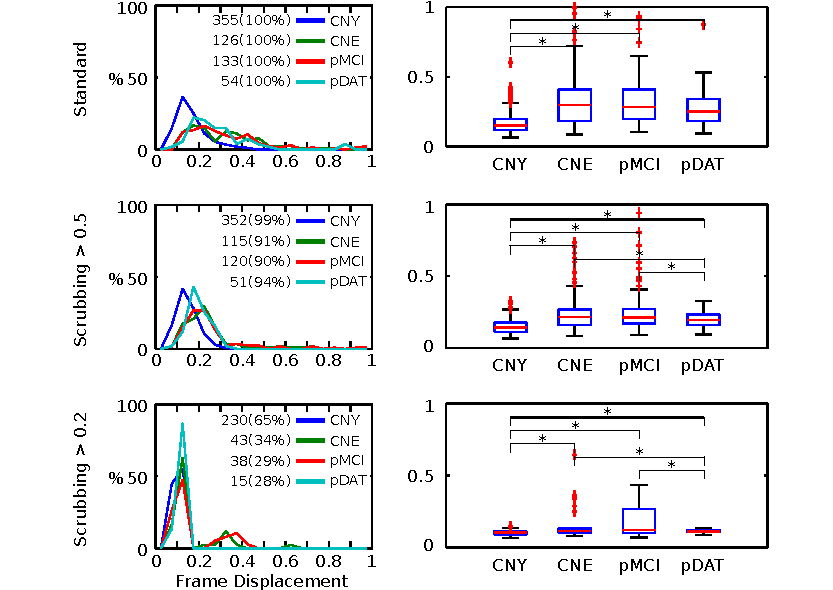
\includegraphics[width=\linewidth]{../figures/figure_fd_distrib.pdf}
\end{center}
\caption{
{\bf Distribution of the frame displacement (FD) for 3 groups (CNE, pMCI, pDAT) when scrubbing is applied at various level (no scrubbing, scrubbing of $FD>0.5$ and scrubbing of $FD>0.2$).}
\label{fig_dist}
\end{figure}

\begin{figure}[!ht]
\begin{center}
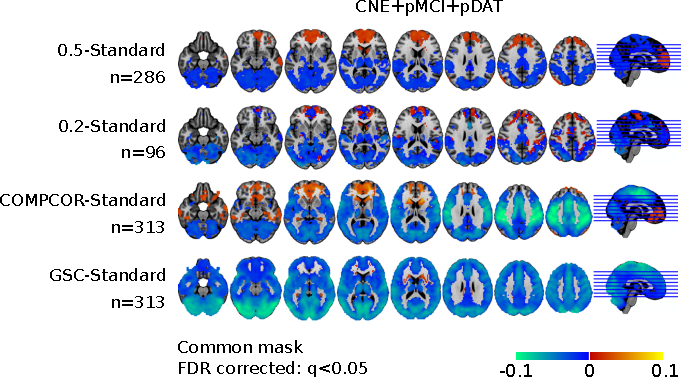
\includegraphics[width=\linewidth]{../figures/figure_comp.pdf}
\end{center}
\caption{
{\bf Differences in functional connectivity for the default mode network (seed in the PCC). On the top the differences in connectivity between all the groups pooled together (CNE,pMCI,pDAT) with and without scrubbing ($FD>0.5$ and $FD>0.2$) (FDR correction $q<0.05$) for all voxels showing a significant effect in at least one of the contrast, the differences are represented without threshold. On the bottom, the differences are represented for each clinical group separately with the same common mask.}
\label{fig_comp}
\end{figure}

\begin{figure}[!ht]
\begin{center}
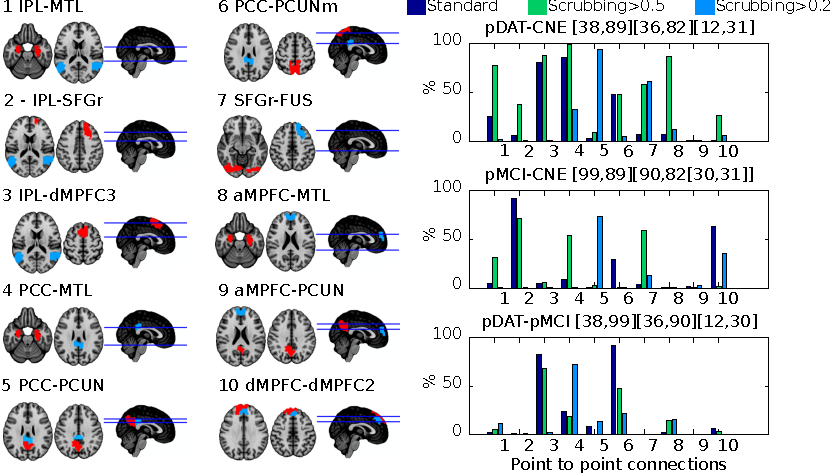
\includegraphics[width=\linewidth]{../figures/p2pdetection.pdf}
\end{center}
\caption{
{\bf On the Left: Seeds from 10 point-to-point connections. PCC (posterior cingulate cortex), PCUN (precuneus), dMPFC (dorsomedial prefrontal cortex), dMPFC2 (dorsomedial prefrontal cortex2), IPL (inferior parietal lobule), SFGr (right superior frontal gyrus), aMPFC (anterior medial prefrontal cortex), PCUNm (precuneus motor), dMPFC3 (dorsmedial prefrontal cortex3), MTL (Mesial temporal lobe). On the right: Detection power of group differences for 3 preprocessing stategy (no scrubbing, scrubbing $FD>0.5$ and scrubbing FD >0.2). The detection power is computed using a t-test of each connection (p<0.05) replicated 10,000 times using random subsamples of 70\% of each group. Explanatory variables included age and gender. Consistent differences for data generated on Philips and Siemens scanners were identified using model averaging (Willer et al., 2010).}
}
\label{fig_p2p}
\end{figure}



\clearpage
\appendix

\section{Functional connectomes}
\label{app_connectome}
Let $\mathcal{P}_i$, an average time series $\mathbf{w}_{i}$ of length $T$ is generated. These average time series are then used to generate a $R\times R$ matrix of functional connectivity $\mathbf{Y}=(y_{i,j})_{i,j=1}^R$, where $R$ is the number of parcels (or resolution):
\begin{equation}
 \label{eq_R}
 y_{ij} = F\left(\textrm{corr}(\mathbf{w}_i,\mathbf{w}_j)\right), \quad F(r) = \frac{1}{2}\log\left(\frac{1-r}{1+r}\right),
\end{equation}
where $\textrm{corr}$ is Pearson's linear correlation coefficient and $F$ is the Fisher's transform. The Fisher's transform is used to stabilize the variance of the estimated correlation coefficient \citep{Anderson1958}. This measure was used for $i\neq j$, but we also included a measure of within-cluster average functional connectivity, that uses the voxel-level time series $\mathbf{w}_v$:
\begin{equation}
y_{ii} = F\left(\frac{1}{\#\mathcal{P}_i(\#\mathcal{P}_i-1)}\sum_{v,v'\in\mathcal{P}_i,v\neq v'} \textrm{corr}(\mathbf{w}_v,\mathbf{w}_{v'})\right).
\end{equation}

\section{Ordinary least square GLM estimation}
\label{app_glm}
We further assume that the coefficients of $\mathbf{E}$ are independent and that $(e_{n,l})_{n=1}^N$ are identically distributed with a zero mean and variance $\sigma_l^2$. Under this hypothesis, the maximum likelihood (ordinary least-squares) estimator of $\mathbf{B}$ is:
\begin{equation}
 \label{eq_lse}
 \hat{\mathbf{B}} = (\mathbf{X}'\mathbf{X})^{-1}\mathbf{X}'\mathbf{Y},
\end{equation}
and the estimation of the variance of the noise is:
\begin{equation}
 \label{var_noise}
 \hat{\sigma}_l^2 = \frac{1}{N-C}\sum_{n=1,\dots,N} \hat{e}_{n,l}^2, \quad \textrm{with} \quad \hat{\mathbf{E}} = \mathbf{Y}-\mathbf{X}\hat{\mathbf{B}}.
\end{equation}
The vector $(\hat{\beta}_{c,l})_{l=1}^L$ is a vectorized connectome of statistical parameters, quantifying the modulation of each connection $l$ by the covariate $c$. This is a direct generalization of the concept statistical parametric map (SPM) that has been widely used in task-based fMRI analysis. Each column of the statistical parametric connectome (SPC) is a actually a SPM, testing the modulation of the functional connectivity of a given seed region with the rest of the brain by the covariate of interest. It is possible to test the signficance of each element of the SPC $\hat{\beta}_{c,l}$ against the null hypothesis $(\mathcal{H}_0)$ of no association (i.e. $\beta_{c,l} = 0$), using a $t$-test:
\begin{equation}
 t_l = (\delta_c'\hat{\mathbf{B}}_l)\left(\hat{\sigma}_l\sqrt{\delta_c'(\mathbf{X}'\mathbf{X})^{-1}\delta_c}\right)^{-1},
\end{equation}
where $\delta_c$ is a contrast (column) vector, with $\delta_{d}$ equals 1 for $(d=c)$ and 0 otherwise. Under $(\mathcal{H}_0)$, the quantity $t_l$ follows a Student's $t$ distribution with $N-C$ degrees of freedom. By comparing $t_l$ with the cumulative distribution function $g_{N-C}$ of the Student's distribution, it is possible to derive the bilateral probability of observing $t_l$ under $(\mathcal{H}_0)$:
\begin{equation}
 p_l = 2 \left( 1-g_{N-C}(|t_l|) \right) .
\end{equation}

\section{Global and group FDR}
\label{app_fdr}
For a given method of selection of significant discoveries, let $D^F$ be the number of false positive and $D^T$ the number of true positive. The FDR $q$ is the mathematical expectation of the ratio between the number of false discoveries and the total number of discoveries $D^F/(D^F + D^T)$ (with the usual convention that $0/0=0$). , i.e. $q\leq \alpha$. Let's assume that the PCE values have been ordered such that $p_{l}\leq p_{l+1}$. The Benjamini-Hochberg (BH) procedure is built on an estimate $\hat{q}(p_l)$ of the false-positive rate equal to $Lp_l/l$. , The BH procedure consists of finding the largest integer $m$ such that $\hat{q}(p_{l})\leq \alpha$ for all $l\leq m$. If such an integer does not exist, there are no discoveries. Otherwise, all connections $l\leq m$ are considered as significant. 
\par
Let us first assume that we know the proportion $\pi_0(i)$ of true negatives in the map associated with the parcel $i$ (oracle case). All the $p$ values in the map are re-weighted based on this proportion (in order to give more weight, or smaller 
$p$, to maps with lots of signal):
\begin{equation}
 \label{eq_weight_GBH}
 p^w_{i,j} = \frac{\pi_0(i)}{1-\pi_0(i)}p_{i,j}.
\end{equation}
Note that, while the initial connectome of $p$ values was symmetric ($p_{i,j} = p_{j,i}$), the weighted matrix of $p^w$-values is not symmetric anymore because the $p^w$-values have been adjusted for the context (number of potential discoveries in the map). A standard (local) BH procedure is then applied within each map $(p^w_{i,j})_{j=1}^R$ with a modified significance level of $\alpha/(1-\pi_0)$, where $\pi_0$ is the global proportion of true negatives equal to $(\sum_{i=1}^R \pi_0(i) )/R$. In the event where $\pi_0(i)$ equals 1, by convention the procedure specifies that no discovery was made with the map associated with parcel $i$. In practice, the proportions $\pi_0(i)$ are unknown and need to be estimated directlty from the data. 

\paragraph{Estimation of the proportion of signal per map} taking the parameters $\mathbf{B}_k$ back into a (connectome) $R\times R$ square form. Two estimators have been put forward in the work of \cite{Hu2010}. The simplest one, called two-stage (TST), is based on the number $\hat{D}^T(i)$ of findings identified by the \textbf{BH-local} procedure in the map $(p_{i,j})_i$, using a modified rejection 
rate of $\alpha/(1-\alpha)$. The estimator $\hat{\pi}^\textrm{TST}_0(i)$ is then simply defined as the ratio $(R-\hat{D}^T(i))/R$. The second estimator is called least-slope (LSL) and was proposed by \cite{Benjamini2001}. Let's assume that the $(p_{ij})_j$ have been sorted in an increasing order as a function of $j$. The LSL estimator is then given by: 
\begin{equation}
 \label{eq_lsl}
 \hat{\pi}^{\textrm{LSL}}_0(i) = \min_j\left(\frac{\lfloor l_{i,j} \rfloor +1}{R},1\right), \quad \textrm{with} \quad l_{i,j} = \frac{R+1-j}{1-p_{i,j}}.
\end{equation}
Two new group FDR procedure can now be defined, both based on the \textbf{GBH} procedure with oracle. The first procedure (\textbf{GBH-TST}) is obtained by replacing $\pi_0(i)$ by $\hat{\pi}^\textrm{TST}_0(i)$, and the second procedure (\textbf{GBH-LSL}) is obtained by replacing  $\pi_0(i)$ by $\hat{\pi}^\textrm{LSL}_0(i)$. As was done with \textbf{BH-global}, those two group procedures control the BH FDR but do not control for the (local) FDR within maps. They can thus be combined with the \textbf{BH-local} procedure. The two resulting algorithms are called \textbf{GBH-TST+local} and \textbf{GBH-LSL+local}.

\section{Generation of statistical parametric connectomes under the global null hypothesis}
Let $\mathbf{Y}^{(s)}$ be the (subject x connections) matrix of individual connectomes at scale $s$ and $\mathbf{X}_{\bar{k}}$ be the reduced model where the $k^\textrm{th}$ covariate has been removed from $\mathbf{X}$. Let $\hat{\mathbf{E}}^{(s)}_{\bar{k}}$ be the residuals of the regression of $\mathbf{X}_{\bar{k}}$ on $\mathbf{Y}^{(s)}$, with associated regression coefficients $\hat{\mathbf{B}}^{(s)}_{\bar{k}}$. The null hypothesis resampling scheme consists of permuting randomly the rows (subjects) of $\hat{\mathbf{E}}^{(s)}_{\bar{k}}$ in order to generate a replication $\hat{\mathbf{E}}^{(s,*)}_{\bar{k}}$ of the residuals. A replication 
of 
the connectome matrix under $(\mathcal{G}_0)$ is then generated by recomposing the linear mixture:
\begin{equation}
 \label{eq_samp_null}
 \hat{\mathbf{Y}}^{(s,*)} = \mathbf{X}_{\bar{k}} \hat{\mathbf{B}}^{(s)}_{\bar{k}} + \hat{\mathbf{E}}^{(s,*)}_{\bar{k}}.
\end{equation}
The estimation procedure is then replicated with the full model $\mathbf{X}$ and $\hat{\mathbf{Y}}^{(s,*)}$ to generate a replication $D^{(*)}_s$ of the number of findings at scale $s$ under $(\mathcal{G}_0)$.
\par
Because the same dataset at native resolution is used to generate all the connectome datasets $(\mathbf{Y}^{(s)})_s$, the samples $D^{(*)}_s$ are not independent. In order to respect these dependencies, for any given replication, the same permutation of the subjects is applied to all of the $(\hat{\mathbf{E}}^{(s)}_{\bar{k}})_s$. The replication of the total number of discoveries $D^{(*)}$ is then simply the sum of $D^{(*)}_s$ for all $s$. This procedure is repeated $B$ times in order to generate $B$ replications $(D^{(*b)})_{b=1}^B$ of the number of discoveries under $(\mathcal{G}_0)$. The Monte-Carlo estimation of the probability to observe a greater number of discoveries than $D$ under $(\mathcal{G}_0)$ is then:
\begin{equation}
 \label{eq_pce_disc}
 \textrm{Pr}(D^{(*)}\geq D | \mathcal{G}_0) \doteq \#\left\{b=1,\dots,B|D^{(*b)}\geq D\right\}/B.
\end{equation}
where $\doteq$ means that the two terms are asymptotically equal as $B$ tends toward infinity. 

%% SUPPLEMENTARY MATERIAL
\clearpage
\pagebreak
\renewcommand{\thefigure}{S\arabic{figure}}
\renewcommand{\thetable}{S\arabic{table}}
\setcounter{figure}{0}
\begin{center}
\emph{Supplementary Material {--} To Scrub Or Not To Scrub: The Impact Of Scrubbing On Resting-­State Connectivity In Alzheimer Progression}\\

\vspace{\baselineskip}Submitted to Neuroimage.\\

\vspace{\baselineskip}C. Dansereau$^{1,3}$,  P. Orban$^{1,2}$, P. Bellec$^{1,3}$\\
\end{center}
$^1$Functional Neuroimaging Unit, Centre de Recherche de l'Institut Universitaire de G\'eriatrie de Montr\'eal\\
$^2$Department of Psychiatry\\
$^3$Department of Computer Science and Operations Research, University of Montreal, Montreal, Quebec, Canada\\

For all questions regarding the paper, please address correspondence to Pierre Bellec, CRIUGM, 4545 Queen Mary, Montreal, QC, H3W 1W5, Canada. Email: pierre.bellec (at) criugm.qc.ca.\\


\pagebreak

\begin{figure}[!ht]
\begin{center}
\includegraphics[width=\linewidth]{../figures/fig_generation_simu.pdf}
\end{center}
\caption{
{\bf Data generation procedure for simulations.} {Etc.} 
}
\label{fig_generation_simu}
\end{figure}


\begin{table}[!ht]
\begin{center}
\includegraphics[width=\linewidth]{../figures/tab_fdr.pdf}
\end{center}
\caption{
{\bf Summary of the empirical false-discovery rate of GLM-connectome (with group or BH FDR), NBS and MDMR on simulations.} {Etc.} 
}
\label{tab_fdr}
\end{table}


\end{document}


